\documentclass[10pt,a4paper]{ctexart}
\usepackage[utf8]{inputenc}
\usepackage{amsmath}
\usepackage{amsfonts}
\usepackage{amssymb}
\usepackage{graphicx}
\usepackage{xcolor}
\usepackage{bm}
\author{吴秉哲}
\title{数值分析上机报告}
\begin{document}
\maketitle
这学期每次的上机报告都按如下格式编写:

每份报告分为几个章节,每个章节分别介绍上机作业中的一题,其中每个
题目又分为以下几个部分:
\begin{enumerate}
\item 问题提出及相关背景知识
\item 问题的理论分析及解决方案
\item 程序的部分设计思路与细节
\item 计算成果与分析
\item 本次上机的反思
\end{enumerate}
每个题目中要求回答的问题均蕴含在问题的理论分析与计算成果分析两部分

在程序方面,都是由C++编写完成(其中用到了自己编写的库:矩阵(Matrix),向量(Vector),以及数值代数的相关算法(linear)),在linux下由g++编译。数据方面
一般使用matlab可视化处理,少部分使用了python。

\section{第五章第一题}
\subsection{问题提出及相关背景知识}
题目给出一个严格对家占优的循环矩阵,要求对$N=2^{10}$用FFT的方法解对应的方程组,并与共轭梯度法比较。
\subsection{问题的理论分析及解决方案}
由于所解方程的系数矩阵为严格对家占优的循环矩阵,则可以推导出其为正定对称矩阵,进而可以使用PCG(预优共轭梯度法)进行数值求解。
又由于其为循环矩阵,由教材的推导,可以使用离散傅立叶变化求解,当矩阵的阶数$N=2^n$时,还可以使用FFT加速。

在本题的上机中,直接选取对角矩阵为预优矩阵。
\subsection{程序设计的思路与细节}
本次上机程序设计的主要难点为FFT算法的实现,我在程序中使用了递归来实现FFT。值得一提FFT的算法可以有两种思路,一种为教材的思路,
还有一种从信号处理的角度来看,可以对所变化向量从频域上划分,也可以作类似的实现。我在我的程序Fourier.h中,对这两种方法都有实现。
\subsection{计算成果与分析}
首先给出题目要求的几个特殊结果,然后列出进一步实验的一些数据,最后对两种方法进行分析。

取$N=2^{10}$时,用FFT解对应方程组所得到的结果达到了机器精度,花费了0.006s。取$N=100,N=150$时,PCG法均在迭代8步以内得到了机器精度
的解。

下面我们看一看进一步的结果。

不难看出所求方程组的精确解为$(0.5,0.5,\cdots,0.5)^T$,而进行实验方法都可以在一定条件下达到机器精度,于是我主要通过控制相同精度,然后

取$2^{n},n=1,2,\cdots,10$为系数矩阵的阶数,观察两种方法所需要的时间,并将其做可视化处理得到了下面一张图表:
\par
\centerline{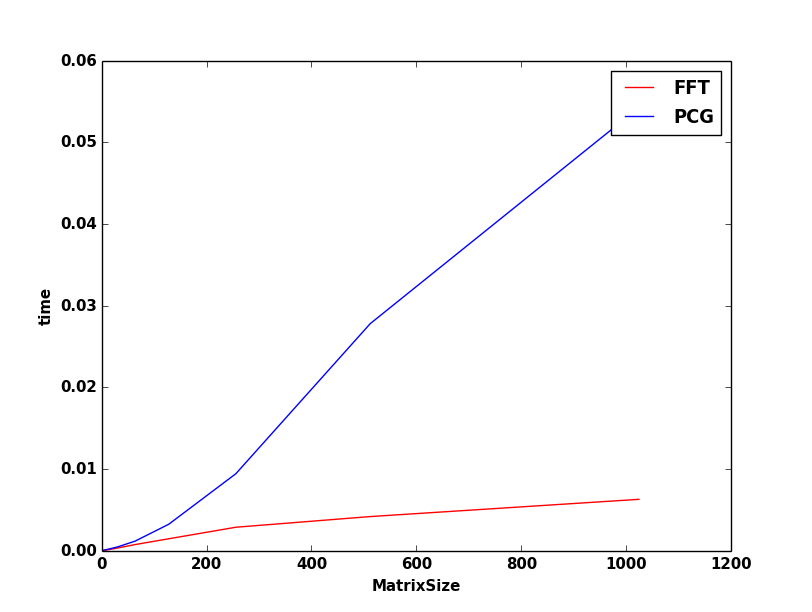
\includegraphics[height=7cm,width=10cm]{fft1.png}}
\par
在上图中,红线表示FFT方法随着N的变化所需时间的变化,而蓝线表示PCG法。
从上图明显可以看出FFT与PCG法所花费时间的差异,共轭梯度法的时间负责度为$O(N^2)$,而FFT为$O(Nlog(N))$,图像与之相符合。
\subsection{本次上机反思}
在这个题的充分感受到了FFT在解某些特殊问题的优势,以后在解决类似问题的时候,如果问题的规模较大,可以优先考虑使用
离散傅立叶变化来解决,进而可以用FFT进行加速。
\section{第五章第二题}
\subsection{问题提出及相关背景知识}
题目给出了两个非周期的具有紧支集的向量,要求计算非周期的卷积。具有紧支集可以得到该向量的分量只有有限个不为0。本题
具有信号处理的学科背景,具体见下一节的分析。
\subsection{问题的理论分析及解决方案}
本题来源于信号处理,信号处理中经常需要求两个离散信号的卷积,但是一般求周期卷积的方法比较简单,信号处理中周期卷积也叫循环卷积。但是我们
在实际问题中常常遇到题目中的这种普通卷积,这时根据信号处理中的循环卷积定理可以将普通卷积的计算转化为循环卷积的计算。

由于本题所给的卷积为两个向量的非周期卷积(教材所给方法为计算循环卷积的情形),所以需要对教材FFT求循环卷积的方法进行一定的修改,具体做法如下:

记$N_0=M+Q-1$,选取大小适当的$n$满足$N=2^n\geq N$,比如在本题条件$Q=200,M=500$时,可以取$N=1024$,这时就可以根据教材的方法计算
$(x_1,x_2,\cdots,x_N)$与$(h_1,h_2,\cdots,h_N)$的周期卷积,然后根据周期卷积定理,所求的的卷积即为题目所求的非周期的卷积的前N个分量,
其余分量为0。

综上,就求得所要求的非周期卷积。
\subsection{计算结果分析}

由上面的推导,在计算推导中出现的周期卷积的时候既可以用FFT来做,也可以使用卷积的定义(教材这里不够严谨,教材给的是循环卷积的定义,应该与一般的卷积区分)。下面先列出计算结果的图($x_n,h_n,(x*h)_n$)的离散图像:
\par
\centerline{\includegraphics[height=5cm,width=12cm]{5.2.png}}
\par
\par
\centerline{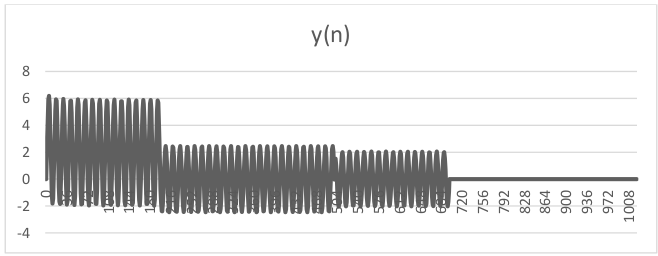
\includegraphics[height=5cm,width=12cm]{5.21.png}}
\par
从上图可以看出最后得到的卷积的图像的特点是信号的能量不停衰减最后到0,这也可以通过对两个信号进行理论上的分析得到。还有一点要提一下的是在电脑上
上机实现FFT变化时涉及到复数运算,我用的是C++ STL模板中的complex模板,这样由于舍入误差的存在,实向量做FFT后最后得到的结果的虚部一般会是一个很小的数,我一般直接舍弃。

下面,我实验了不同大小的$M,Q$,然后比较两种方法在时间上的差异,最后如上题一样绘制了图像,结果如下:
\par
\centerline{\includegraphics[height=7cm,width=10cm]{../vim/5.2.png}}
\par
从上面可以看出FFT方法在花费时间上巨大的优势。
\section{第五章第三题}
\subsection{问题提出及相关背景知识}
这个问题还是来源与信号处理中消除白噪声问题。原题给出一个信号$f(t)$,题目要求做这样的处理:将原信号做离散傅立叶变化后,去掉其中的
高频项,然后做傅立叶反变化,得到一个新信号。题目要求对比原信号图像与新得到的信号的图像的差别。
\subsection{问题理论分析及相关背景知识}
这个问题程序实现起来比较容易。主要要理解它背后的思想,即从消除信号的噪声的角度,来理解离散傅立叶变换在其中起到的作用。

首先我们将输入信号做频谱变化(即第一次FFT),去掉其中的噪声,由信号处理方面的知识,噪声即为做变换后的高频部分,所以过滤掉高频
部分就可以达到消除噪声的效果,而教材题目给的方法为给定m,令高频部分为0,这其实就是信号处理中截断函数的另一种提法下面我们来看看这种方法的实际效果。
\subsection{计算结果分析}
首先我们用Python画出原始信号的图像,如下:
\par
\centerline{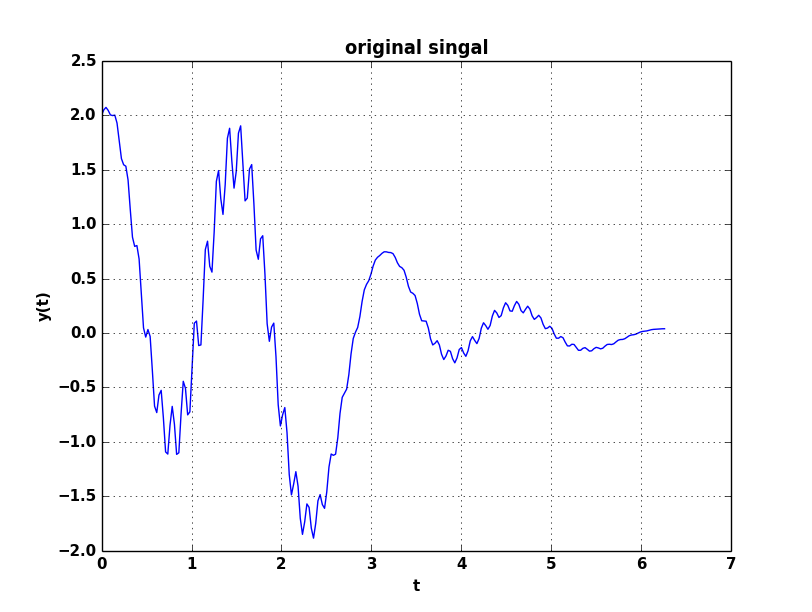
\includegraphics[height=7cm,width=12cm]{singal0.png}}
\par
从上图可以看出,信号受噪声的影响还是很明显的。下面我们来看看处理过后的信号的图像(图像为题目中$m=6$时):
\par
\centerline{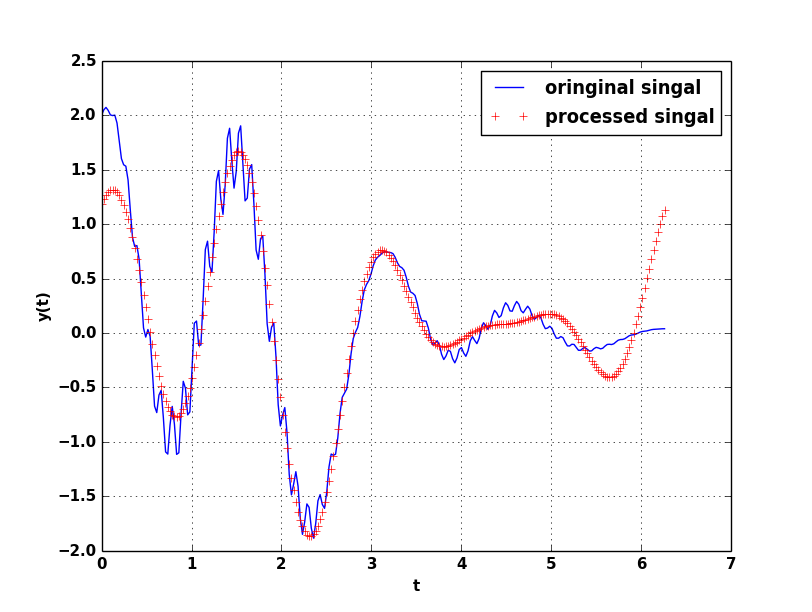
\includegraphics[height=7cm,width=12cm]{singal1.png}}
\par
由对比图可以发现此种方法消除噪声的效果特别明显.

进一步实验,改变m的值,可以发现当m越大时,所得的信号与原始信号越接近,也就是消除噪声的效果减弱了,由于篇幅原因,就不再画图对比了。

以上就是整个信号消噪的过程,在以后实际应用中,还可能需要构造不同的截断函数对信号处理,这就不属于数值分析的范畴了。
\section{第六章第一题}
\subsection{问题提出及相关背景知识}
题目给定一个初值问题,要求使用欧拉方法与改进的欧拉方法进行数值求解,并对比相应的计算结果。
\subsection{问题理论分析及解决方案}
方程可以直接使用我自己编写的常微分方程数值算法库$ode_solve.h$求解,比较简单。
\subsection{程序设计思路}
本次充分实现了面向对象编程的思想,将整个常微分方程组作为一个类来实现,类成员包括了初值与结束值,类函数即为
各种数值格式,比如四阶Runge-Kutta。在实际上机体验中,我感觉这样的写法使整个程序变得简洁,并能够迅速定位错误,而且这样的代码重用性大大提高。
\subsection{计算结果}
根据题目所给的常微分方程,容易求得它的精确解为$\dfrac{1}{x}tan(-\dfrac{\pi}{4}-ln(x))$,这样我们既可以对比Euler法与改进Euler法的计算结果与方程精确解的差别。下面
分步长$h=0.0,0.01.0.001$三种情况,给出对应的计算结果:
\par
\centerline{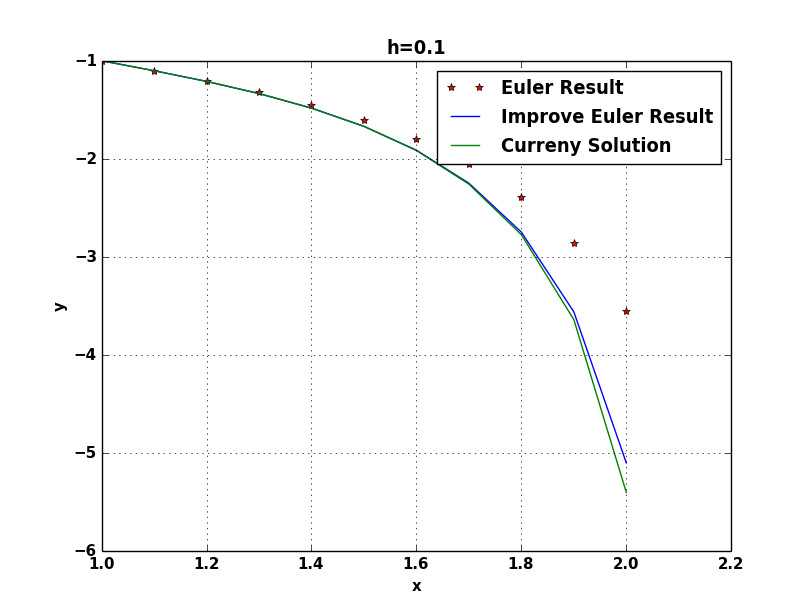
\includegraphics[height=7cm,width=14cm]{0.1h.png}}
\par
\par
\centerline{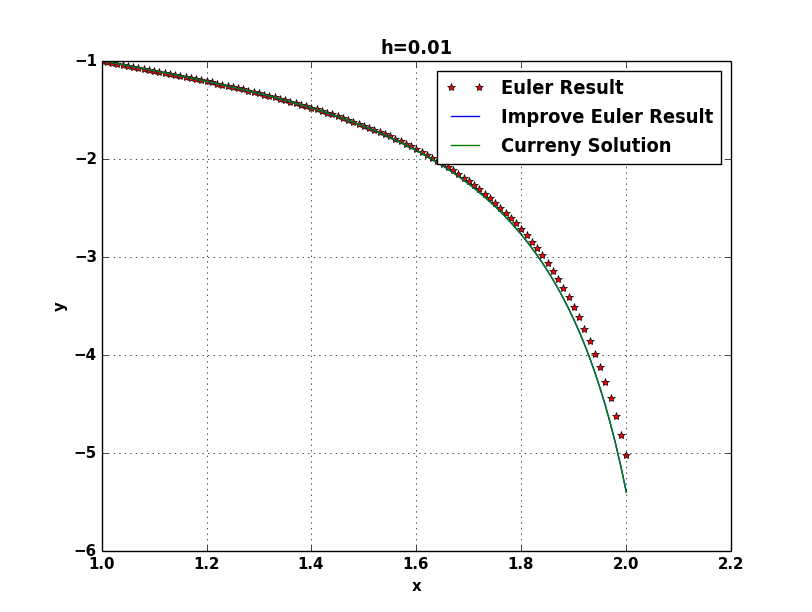
\includegraphics[height=7cm,width=14cm]{0.01h.png}}
\par
\par
\centerline{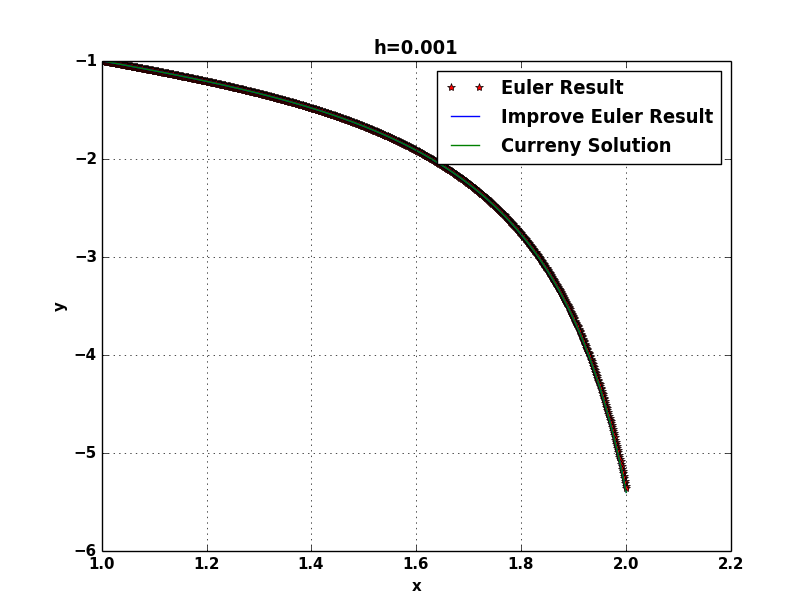
\includegraphics[height=7cm,width=14cm]{0.001h.png}}
\par
由上面三种情况的计算结果可以看出,在$h=0.1$时,改进的Euler法与精确解已经很靠近,但Euler法的计算结果在靠近右端点
的过程中与精确解偏离,随着h的减小,两种方法的计算结果也越来越精确。由这个过程,可以看出改进欧拉法相较与普通欧拉法的
好处,它相当于在计算过程中不断矫正以前的计算值,这也是这种方法比较精确的原因。
\section{第六章第二题}
\section{第六章第四题}
\subsection{问题提出及相关背景知识}
本题要求用数值算法求解洛伦兹方程组,并改变初始值与方程参数,观察所得到计算结果的不同之处。在开始理论分析
之前,我先把我查阅资料所获得的背景知识列在下面,这也对我们求解该方程有一定的启发意义。

美国气象学家洛伦兹(E.N.Lorenz,)是混沌理论的奠基者之一。他在使用计算机模拟天气时意外发现,对于天气系统,哪怕初始条件的微小改变也会显著影响运算结果。随后,他在同事工作的基础上化简了自己先前的模型,得到了有3个变量的一阶微分方程组,由它描述的运动中存在一个奇异吸引子,即洛伦兹吸引子。

洛伦兹方程组是基于流体力学中的Navier-Stokes方程、热传导方程和连续性方程构建的,属于耗散系统。相空间中,耗散系统的终态都将收缩到吸引子的状态上。但对平庸吸引子来说,无论初值如何,终值只有一个,而奇异吸引子却是无数个点的集合,对初值极端敏感。
洛伦兹的工作结果最初在1963年发表,论文题目为Deterministic Nonperiodic Flow,发表在Journal of the Atmospheric Sciences杂志上。

在洛伦兹原始的工作中,x表示的是对流的翻动速率,y正比于上流与下流液体温差,z是垂直方向的温度梯度。式中三个参数$\sigma$(Prandtl数)、$\beta$和$\rho$(Rayleigh数)可任取大于0的数值。常用的组合是$\sigma=10$,$\beta=8/3$,而令$\rho$取不同数值。$\rho=28$时有混沌现象,奇异吸引子出现

\subsection{问题的理论分析及解决方案}
我们从上面的背景知识已经大概了解到这个方程组的意义,以及我们在数值试验时,应该如何去选取初始值与参数。

在对这个方程组的求解中,我主要使用了改进的Euler法,着重于观察方程的数值计算结果有哪些数值特点。
\subsection{计算成果分析}
首先,在题目给定方程参数条件下,尝试了初值(t=0)为(0,0,0)的情况,由于在初值点所有导数都是 0,故无论 t 怎样变化,(x,y,z)恒为(0,0,0).

然后我们改变初值为(0.001,0,0),此时出现了很大变化,见下方左图。t 较小时
有一定的周期性,其后这个周期性被打破,并且三条函数曲线的趋势有无界的倾向。我将对应计算出来的$x(t),y(t),z(t)$的图像画在下面:
\par
\centerline{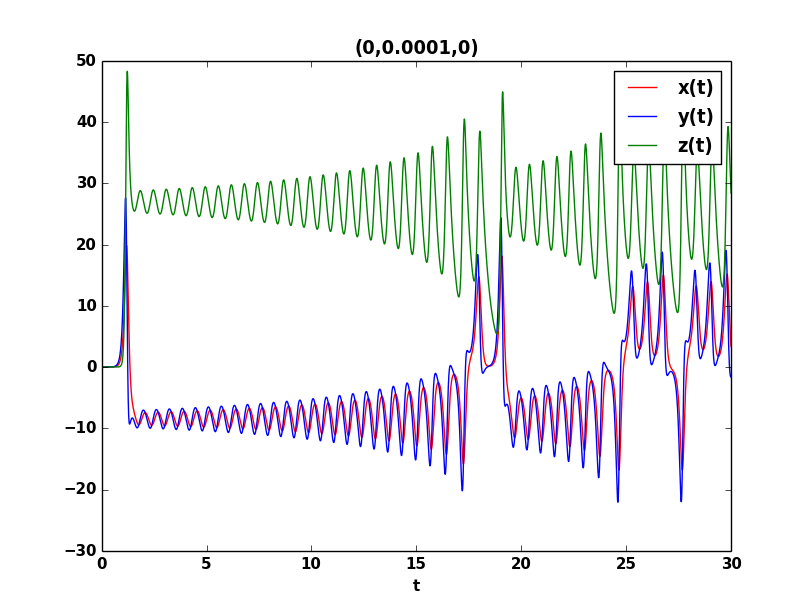
\includegraphics[height=7cm,width=12cm]{lorenz2d1.png}}
\par
当在同样的方程参数条件下(即题目所给的$\delta=10,\rho=28,\beta=8/3$)的情况下取初值分别为$(0,0,0.001)$与$(0,0.001,0)$所得到的计算结果
如下图:
\par
\centerline{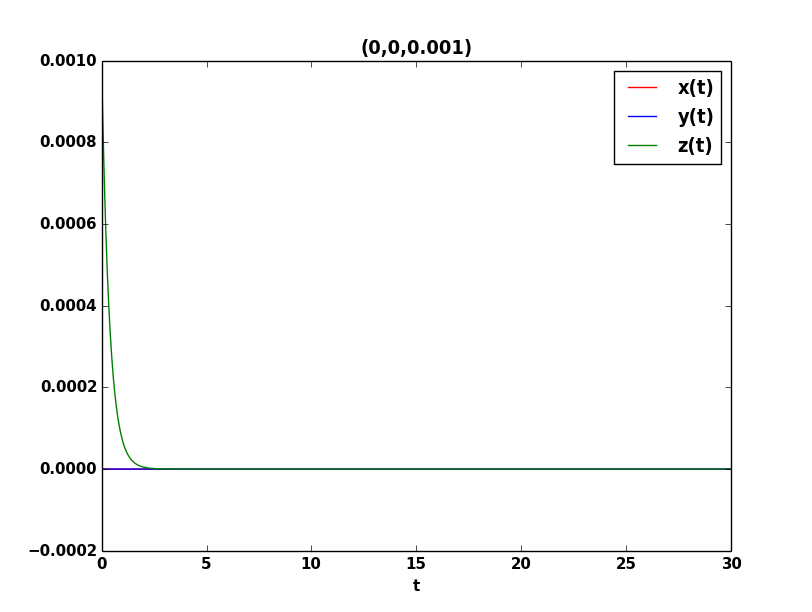
\includegraphics[height=7cm,width=12cm]{lorenz2d2.png}}
\par
\par
\centerline{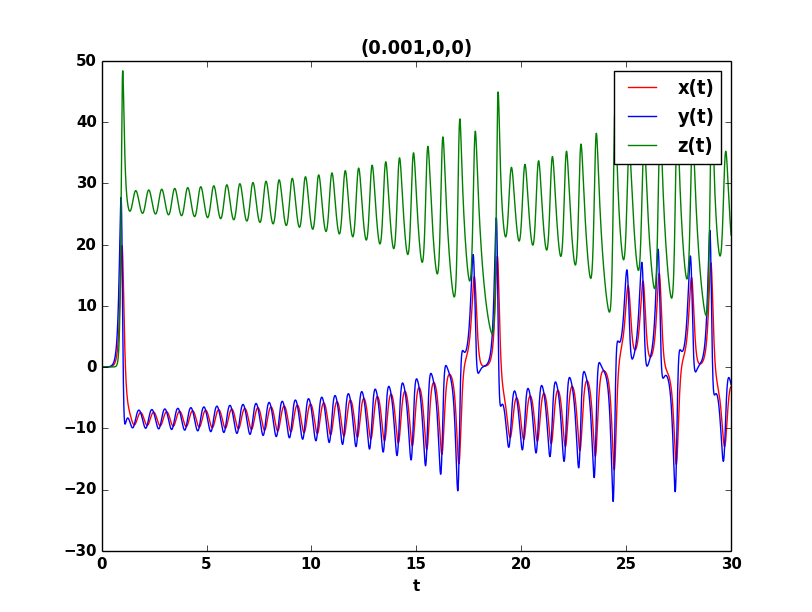
\includegraphics[height=7cm,width=12cm]{lorenz2d3.png}}
\par
有上面的结果可以看出当初值取$(0,0,0.001)$时,解的曲线随着t想无穷趋近时,都趋向于0,而当初值取$(0,0.001,0)$时,解的形态与
最开始的情况类似,只不过振动的方式发生了一些小的变化。

然后继续固定方程的参数,取初值为$(1,1,1)$,得到了振动比较有周期的图像(但是能量在变化),且有趋于无穷的趋势:
\par
\centerline{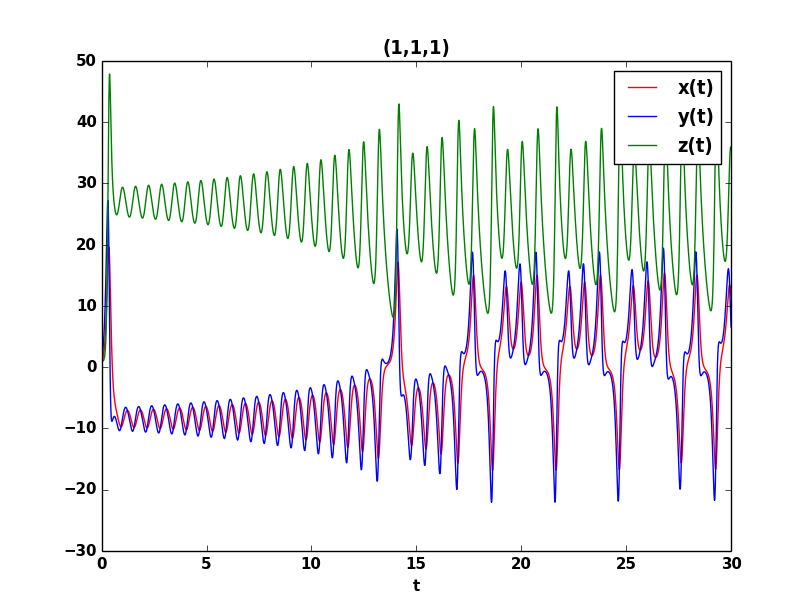
\includegraphics[height=7cm,width=12cm]{lorenzh111.png}}
\par

\section{第六章第五题}
\subsection{问题提出及相关背景知识}
本题要求解一个一阶偏微分方程(给定了初值与周期边界条件):
\begin{equation*}
\dfrac{\partial u}{\partial t}+\dfrac{\partial u}{\partial x}=0
\end{equation*}
这个方程来源于解波动方程时,得到的一个一阶线性方程,可以用特征线法求得它的解析解:
\begin{equation*}
u(x,t)=sin(x-t)
\end{equation*}
\subsection{问题理论分析及解决方案}
观察所给方程特点,发现我们可以将其转化为常微分方程组,具体做法如下:

首先对x离散,在本题的实际计算时,我选择将区间100等分,则当固定x时,$u(x,t)$变为关于t的函数,
对应的方程化为:
\begin{equation*}
    \dfrac{\partial u_i}{\partial t}+\dfrac{u_{i+1}+u_{i-1}}{2h}=0
\end{equation*}
其中h为划分x的步长

这样我们就得到了一个常微分方程组,于是可以利用我们已知的数值格式求解,我在求解时还对t取了一个界,实际上为了避免麻烦,可以直接
将$u(x,t)$作为周期函数处理.
\subsection{计算结果分析}
由于计算结果的数据量较大,我就不将其用表格列出.通过试验我们发现将x与t的步长都取$h$,然后将试验$h=0.01,0.001$时,欧拉法与
二阶Runge-kutta法均不收敛,在刚开始的时候计算结果与精确值偏离不远,但是随着迭代的次数增多,解偏离精确值越来越远,这说明
了我选取的步长不在这个方法的稳定域内,后来试验了其他步长,还是不能使这两种方法收敛,所以试验了另外两种方法。下面是这两种方法
的结果(三阶与四阶):
首先给出精确解的曲面图像:
\par
\centerline{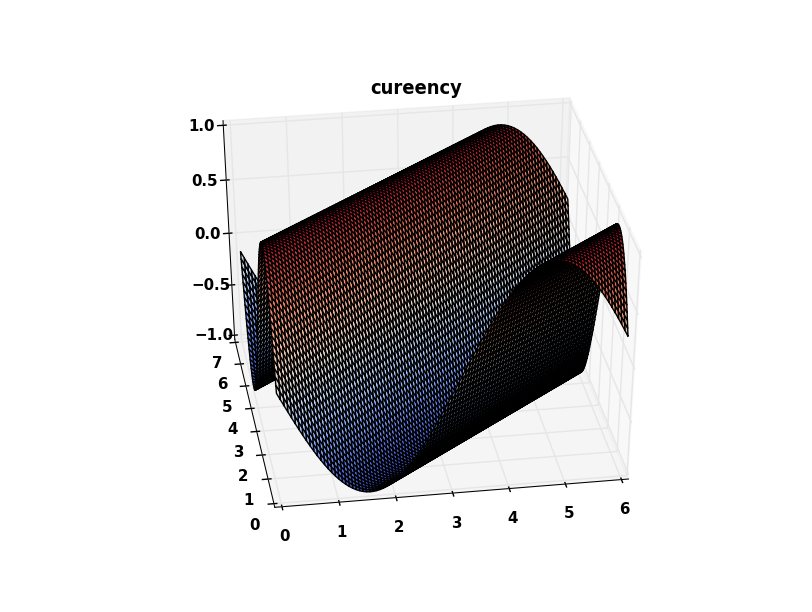
\includegraphics[height=8cm,width=14cm]{6.5.png}}
\par
三级三阶:
\par
\centerline{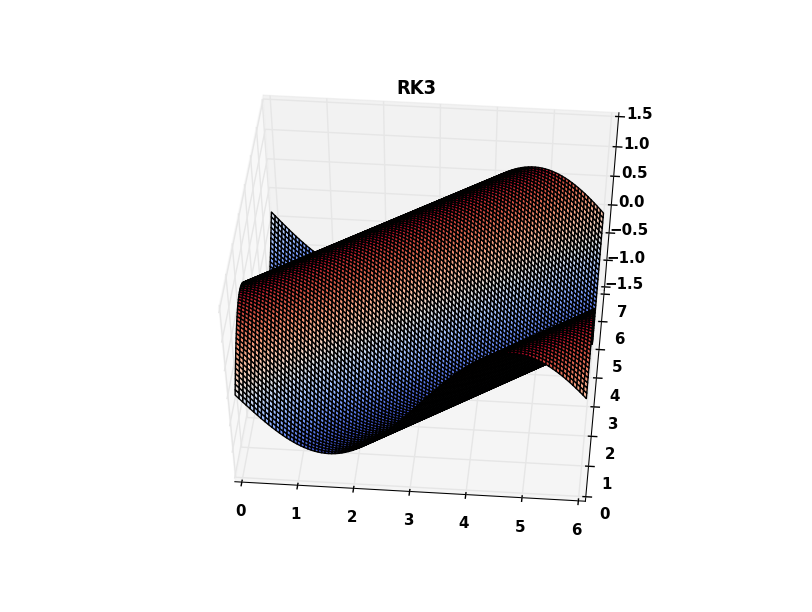
\includegraphics[height=8cm,width=14cm]{6.5.3.png}}
\par
四阶Runge-Kutta:
\par
\centerline{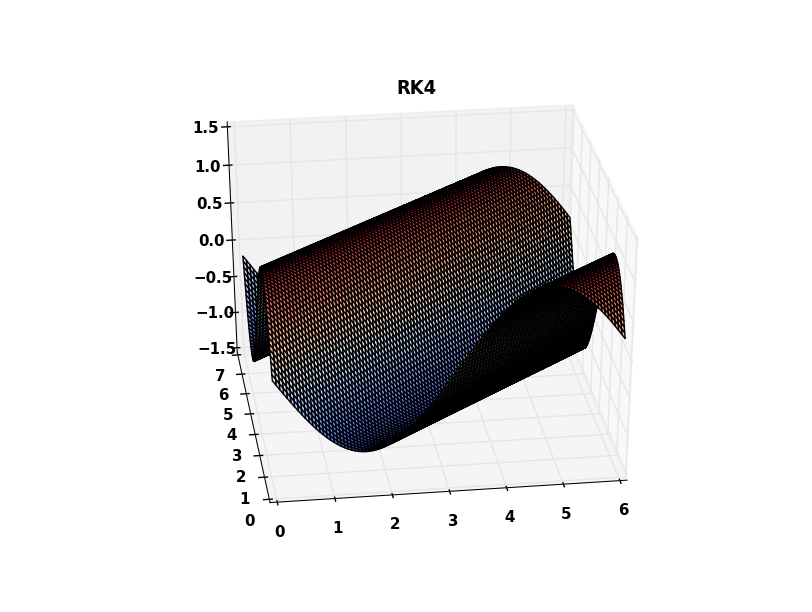
\includegraphics[height=8cm,width=14cm]{6.5.4.png}}
\par
由于计算机舍入误差的关系,两种数值格式在个别点的计算结果都超过了1,这导致了上面图像中z轴的范围超出了1,不过从数据的
整体估计,这两种方法还是基本符合精度要求。
\end{document}
